\documentclass{assignment}
\UsingEnglish
\ProjectInfos*{Intro to Communication System}{EE140}{Fall, 2020}{Assignment 4}{Due time : 10:15, Oct 16, 2020 (Friday)}{陈稼霖}{45875852}
\begin{document}
\begin{prob}[Different Analog Modulation Schemes, 20 pts]
    Using the massage signal $m(t)=10\cos 10\pi t$ and modulation carrier $C(t)=2\cos 200\pi t$, determined signals (time domain expression) for the following methods of modulation, and draw the spectrum of the modulation signals.
    \begin{itemize}
        \item[a)] Double-sideband-suppressed carrier (DSB-SC) modulation.
        \item[b)] Double-sideband, Large carrier (DSB-LC) modulation with modulation index $a=0.1$.
        \item[c)] Single-sideband (SSB) modulation with upper sideband retained.
        \item[d)] Vestigial-sideband (VSB) modulation with following VSB filter $H(f)$ in Figure \ref{Assignment-4-Problem-1}.
    \end{itemize}
    \begin{figure}[h]
        \centering
        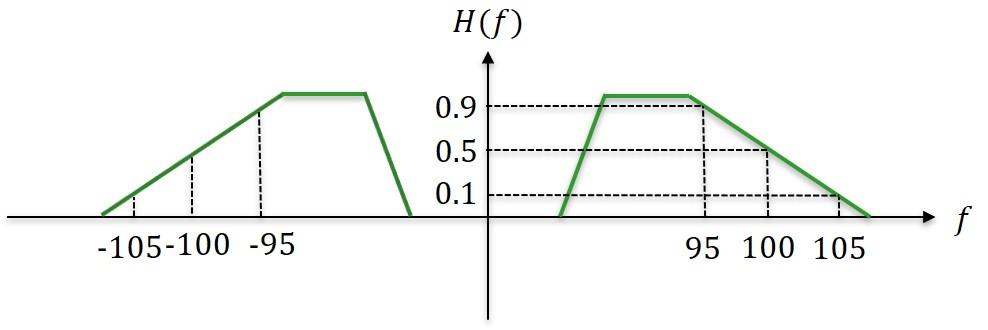
\includegraphics[width=.5\columnwidth]{Assignment-4-Problem-1.jpg}
        \caption{}
        \label{Assignment-4-Problem-1}
    \end{figure}
\end{prob}
\begin{sol}
    \begin{itemize}
        \item[a)] The modulated signal of DSB-SC modulation is
        \begin{align}
            x_c(t)=m(t)C(t)=20\cos(10\pi t)\cos(200\pi t)=20\cos(10\pi t)\cos(200\pi t)=10[\cos(190\pi t)+\cos(210\pi t)].
        \end{align}
        Its spectrum is
        \begin{align}
            X_c(f)=\mathscr{F}[x_c(t)]=5[\delta(f-95)+\delta(f+95)+\delta(f-105)+\delta(f+105)],
        \end{align}
        as shown in figure \ref{Assignment-4-Problem-1-1}.
        \item[b)] The modulated signal of DSB-LC modulation with modulation index $a=0.1$ is
        \begin{align}
            \notag x_c(t)=&2\left[1+a\frac{m(t)}{\abs{\min[m(t)]}}\right]\cos(200\pi t)\\
            \notag=&2\left[1+0.1\frac{10\cos(10\pi t)}{10}\right]\cos(200\pi t)\\
            \notag=&2\cos(200\pi t)+0.2\cos(10\pi t)\cos(200\pi t)\\
            =&2\cos(200\pi t)+0.1[\cos(190\pi t)+\cos(210\pi t)].
        \end{align}
        Its spectrum is
        \begin{align}
            X_c(f)=\delta(f-100)+\delta(f+100)+0.05[\delta(f-95)+\delta(f+95)+\delta(f-105)+\delta(f+105)].
        \end{align}
        as shown in figure \ref{Assignment-4-Problem-1-2}.
        \item[c)] The Hilbert transform of the message signal is
        \begin{align}
            \hat{x}(t)=10\sin(10\pi t).
        \end{align}
        The modulated signal of SSB modulation with upper sideband retained is
        \begin{align}
            \notag x_c(t)=&\frac{1}{2}2m(t)\cos(200\pi t)-\frac{1}{2}2\hat{m}(t)\sin(200\pi t)\\
            \notag=&10\cos(10\pi t)\cos(200\pi t)-10\sin(10\pi t)\sin(200\pi t)\\
            =&10\cos(210\pi t).
        \end{align}
        Its spectrum is
        \begin{align}
            X_c(f)=5[\delta(f-105)+\delta(f+105)],
        \end{align}
        as shown in figure \ref{Assignment-4-Problem-1-3}.
        \item[d)] The spectrum of the message signal is
        \begin{align}
            M(f)=\mathscr{F}[m(t)]=5[\delta(f-5)+\delta(f+5)].
        \end{align}
        The spectrum of the signal of VSB modulation with VSB filter $H(f)$ is Figure \ref{Assignment-4-Problem-1} is
        \begin{align}
            \notag X_c(f)=&[M(f-100)+M(f+100)]H(f)\\
            \notag=&5[\delta(f-105)+\delta(f-95)+\delta(f+95)+\delta(f+105)]H(f)\\
            =&0.5\delta(f-105)+4.5\delta(f-95)+4.5\delta(f+95)+0.5\delta(f+105),
        \end{align}
        as shown in figure \ref{Assignment-4-Problem-1-4}.
        The modulated signal of VSB is
        \begin{align}
            x_c(t)=\mathscr{F}^{-1}[X_c(f)]=9\cos(190\pi t)+\cos(210\pi t).
        \end{align}
        \begin{figure}[h]
            \centering
            \subfigure[DSB-SC]{
                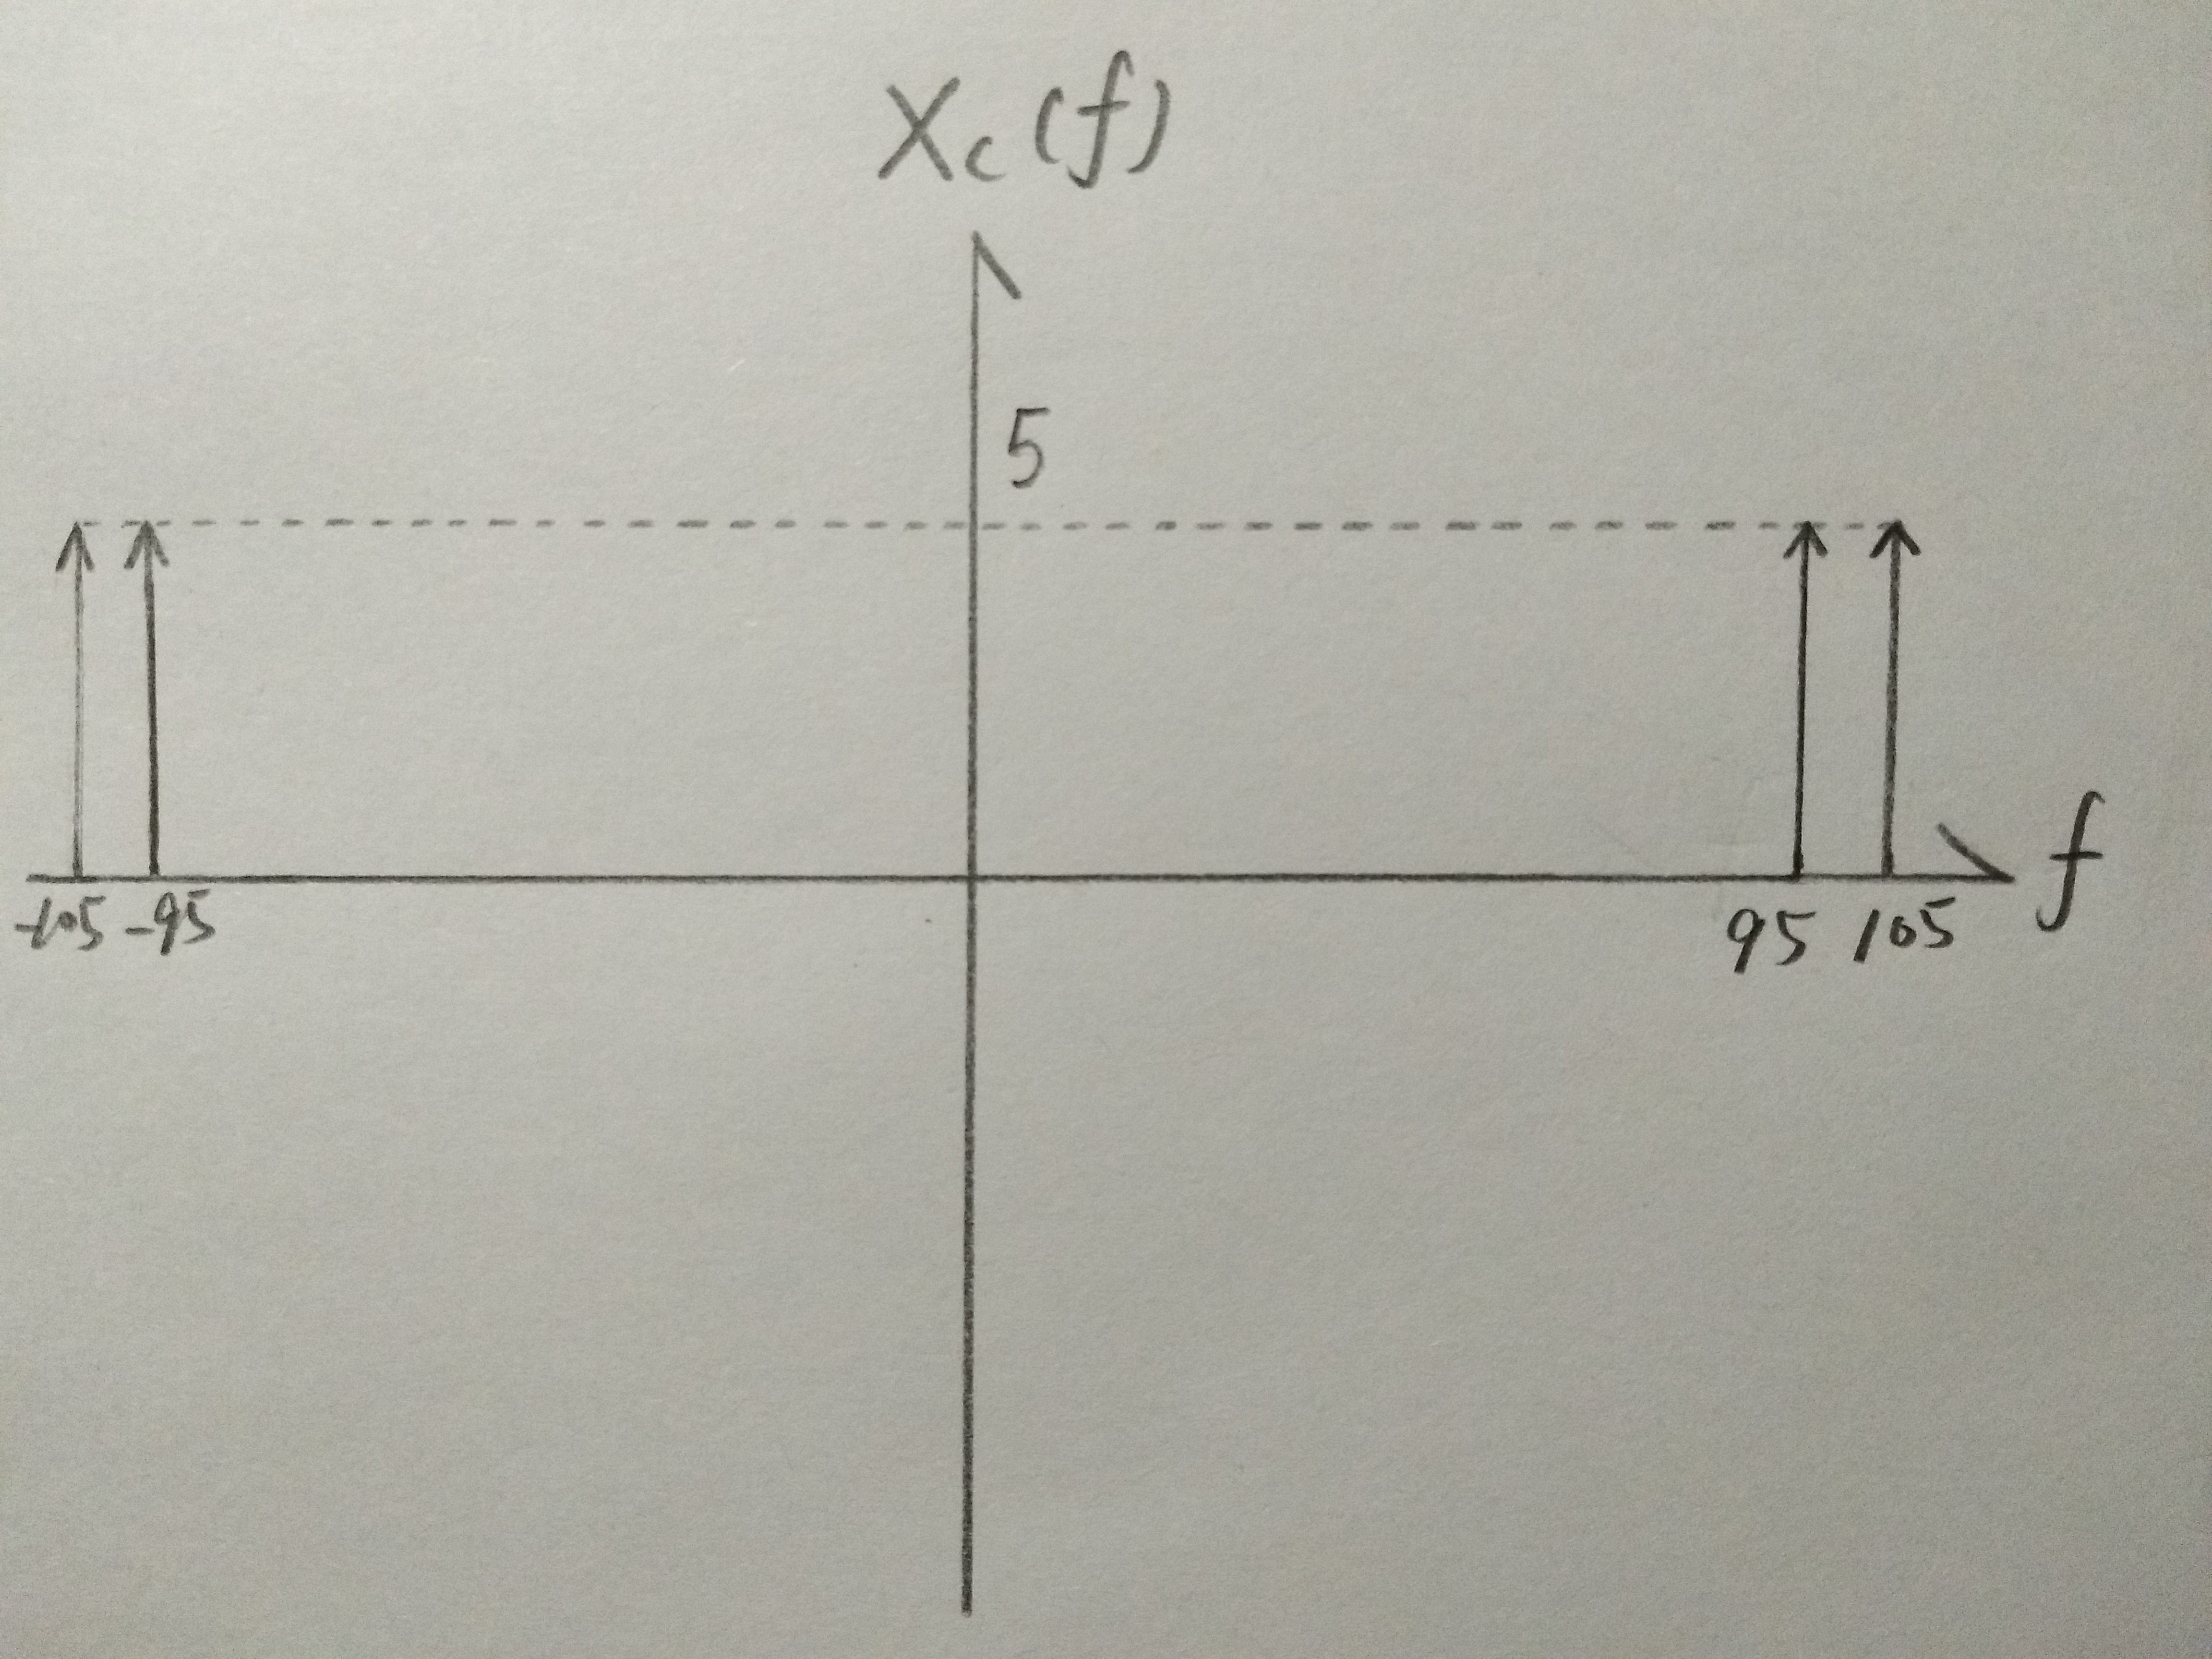
\includegraphics[width=.45\columnwidth]{Assignment-4-Problem-1-1.jpg}
                \label{Assignment-4-Problem-1-1}
            }
            \subfigure[DSB-LC]{
                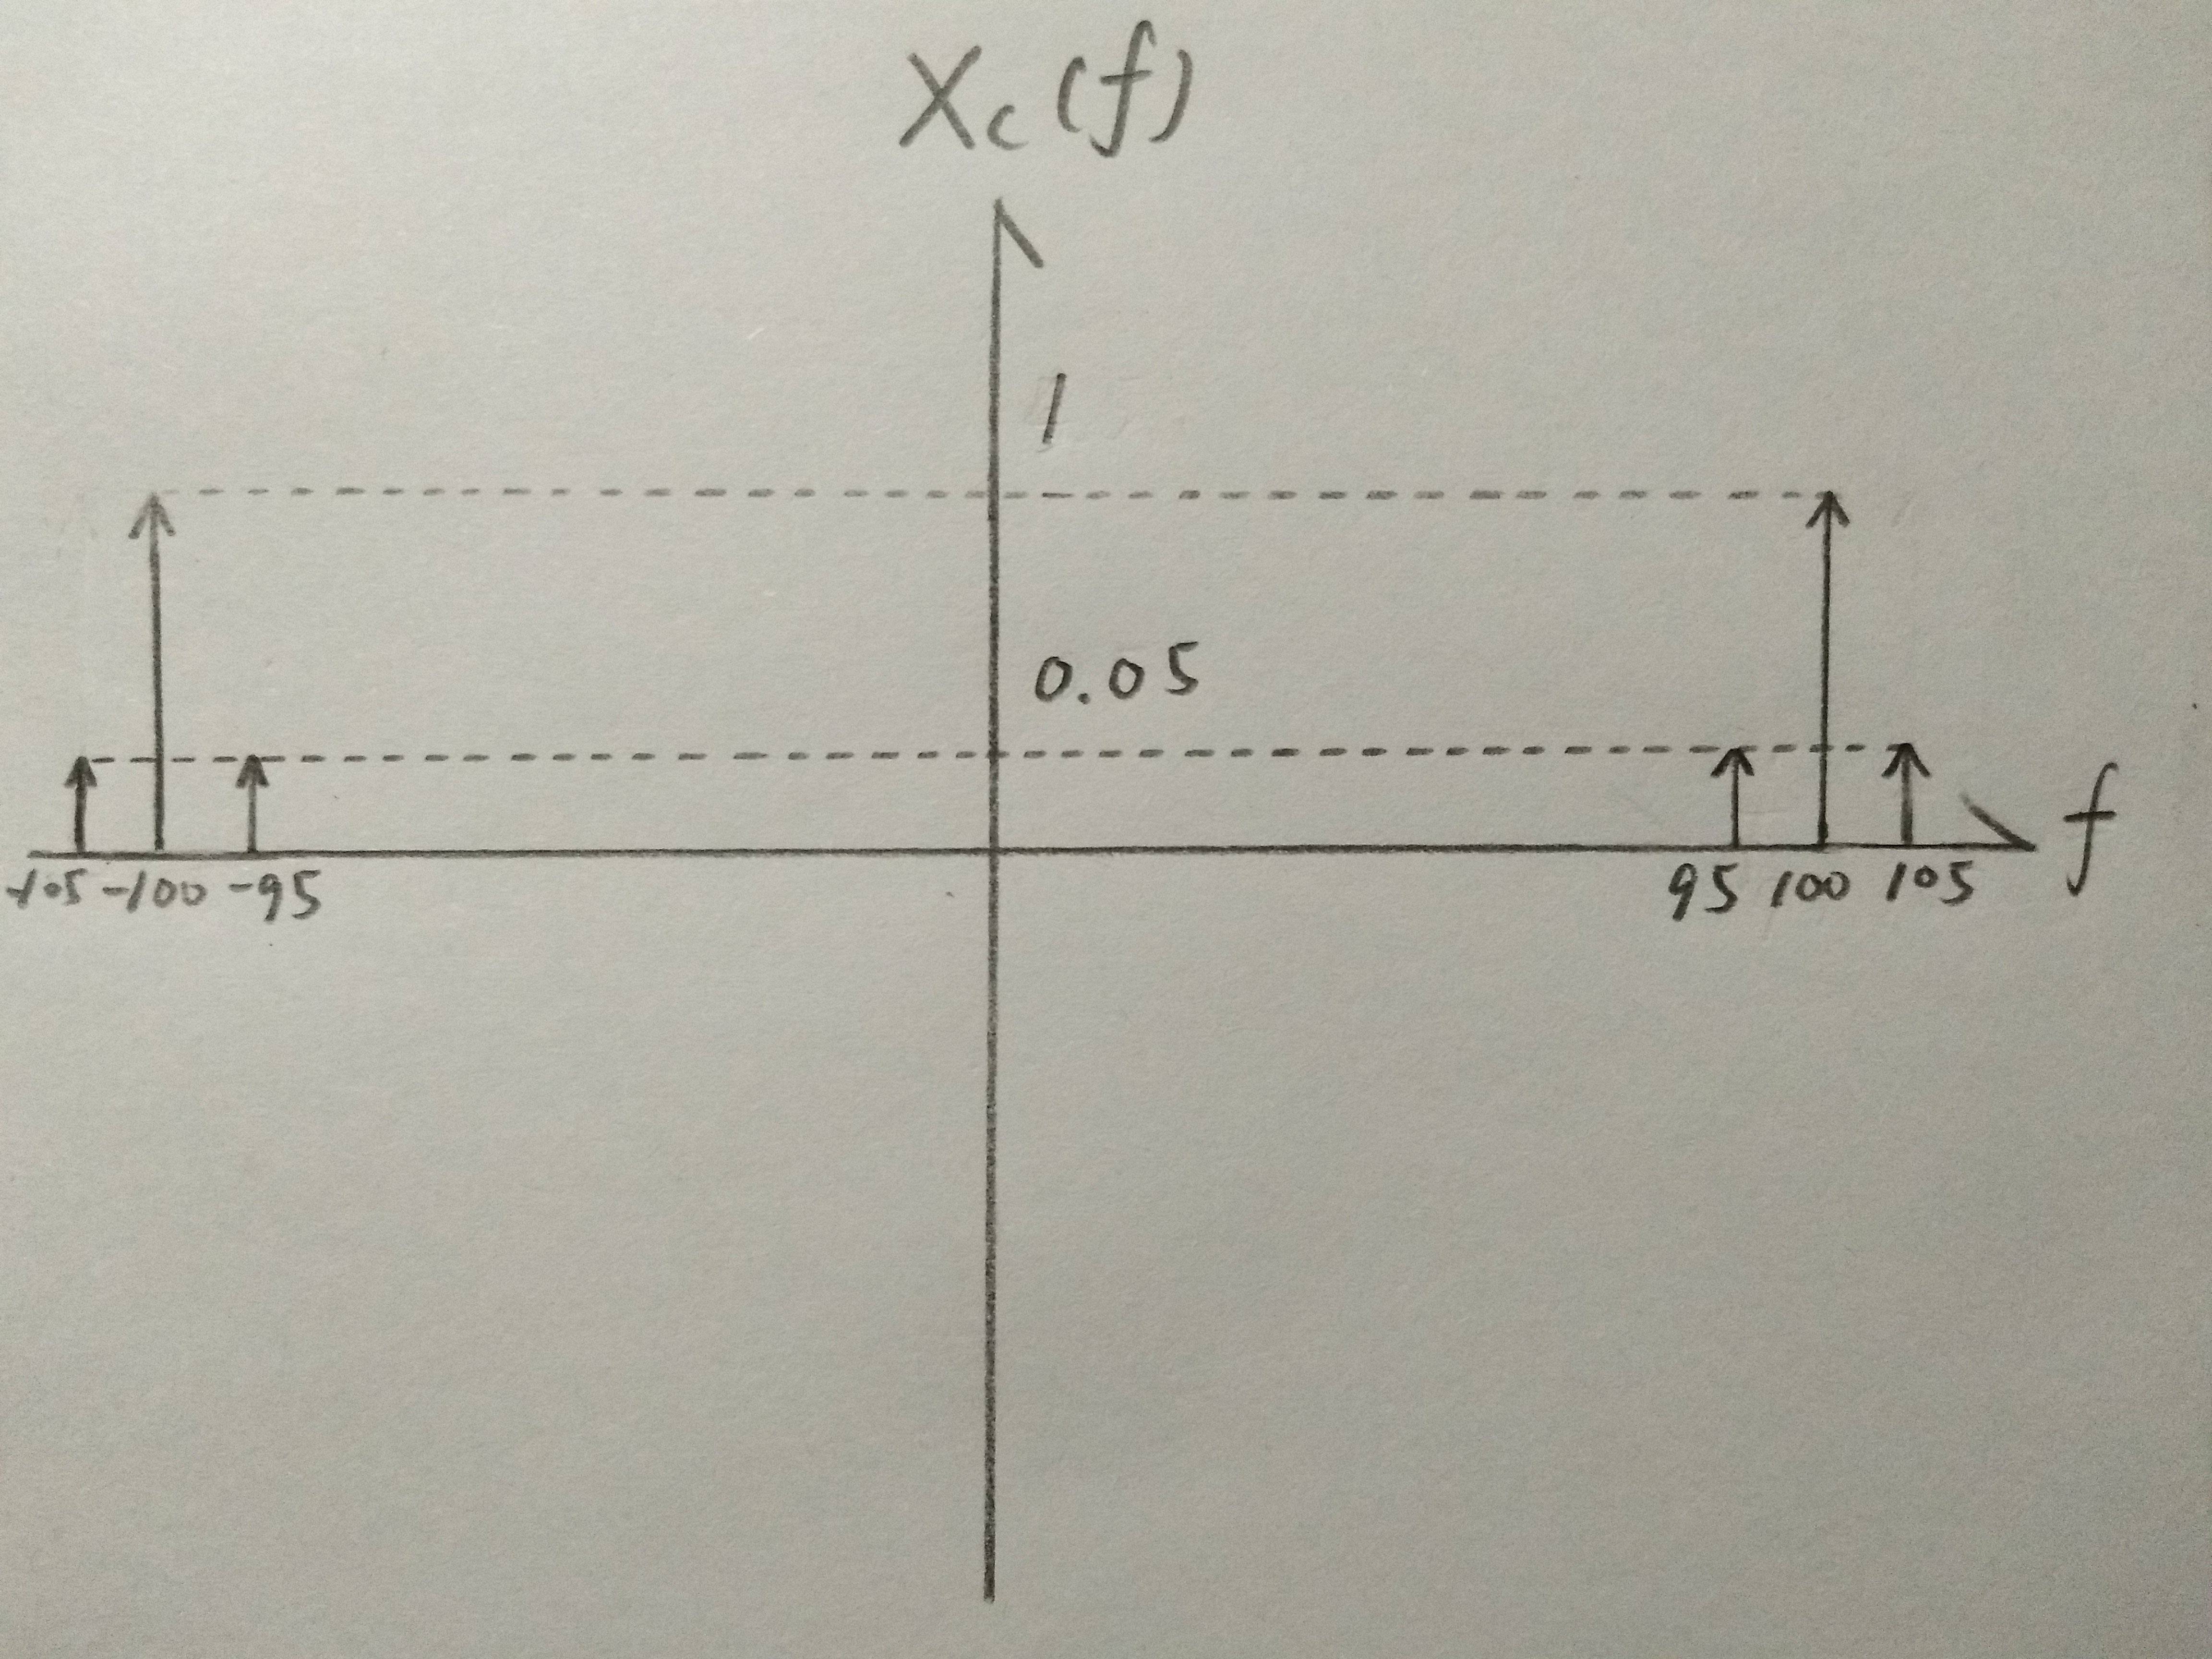
\includegraphics[width=.45\columnwidth]{Assignment-4-Problem-1-2.jpg}
                \label{Assignment-4-Problem-1-2}
            }
            \subfigure[DSB-LC]{
                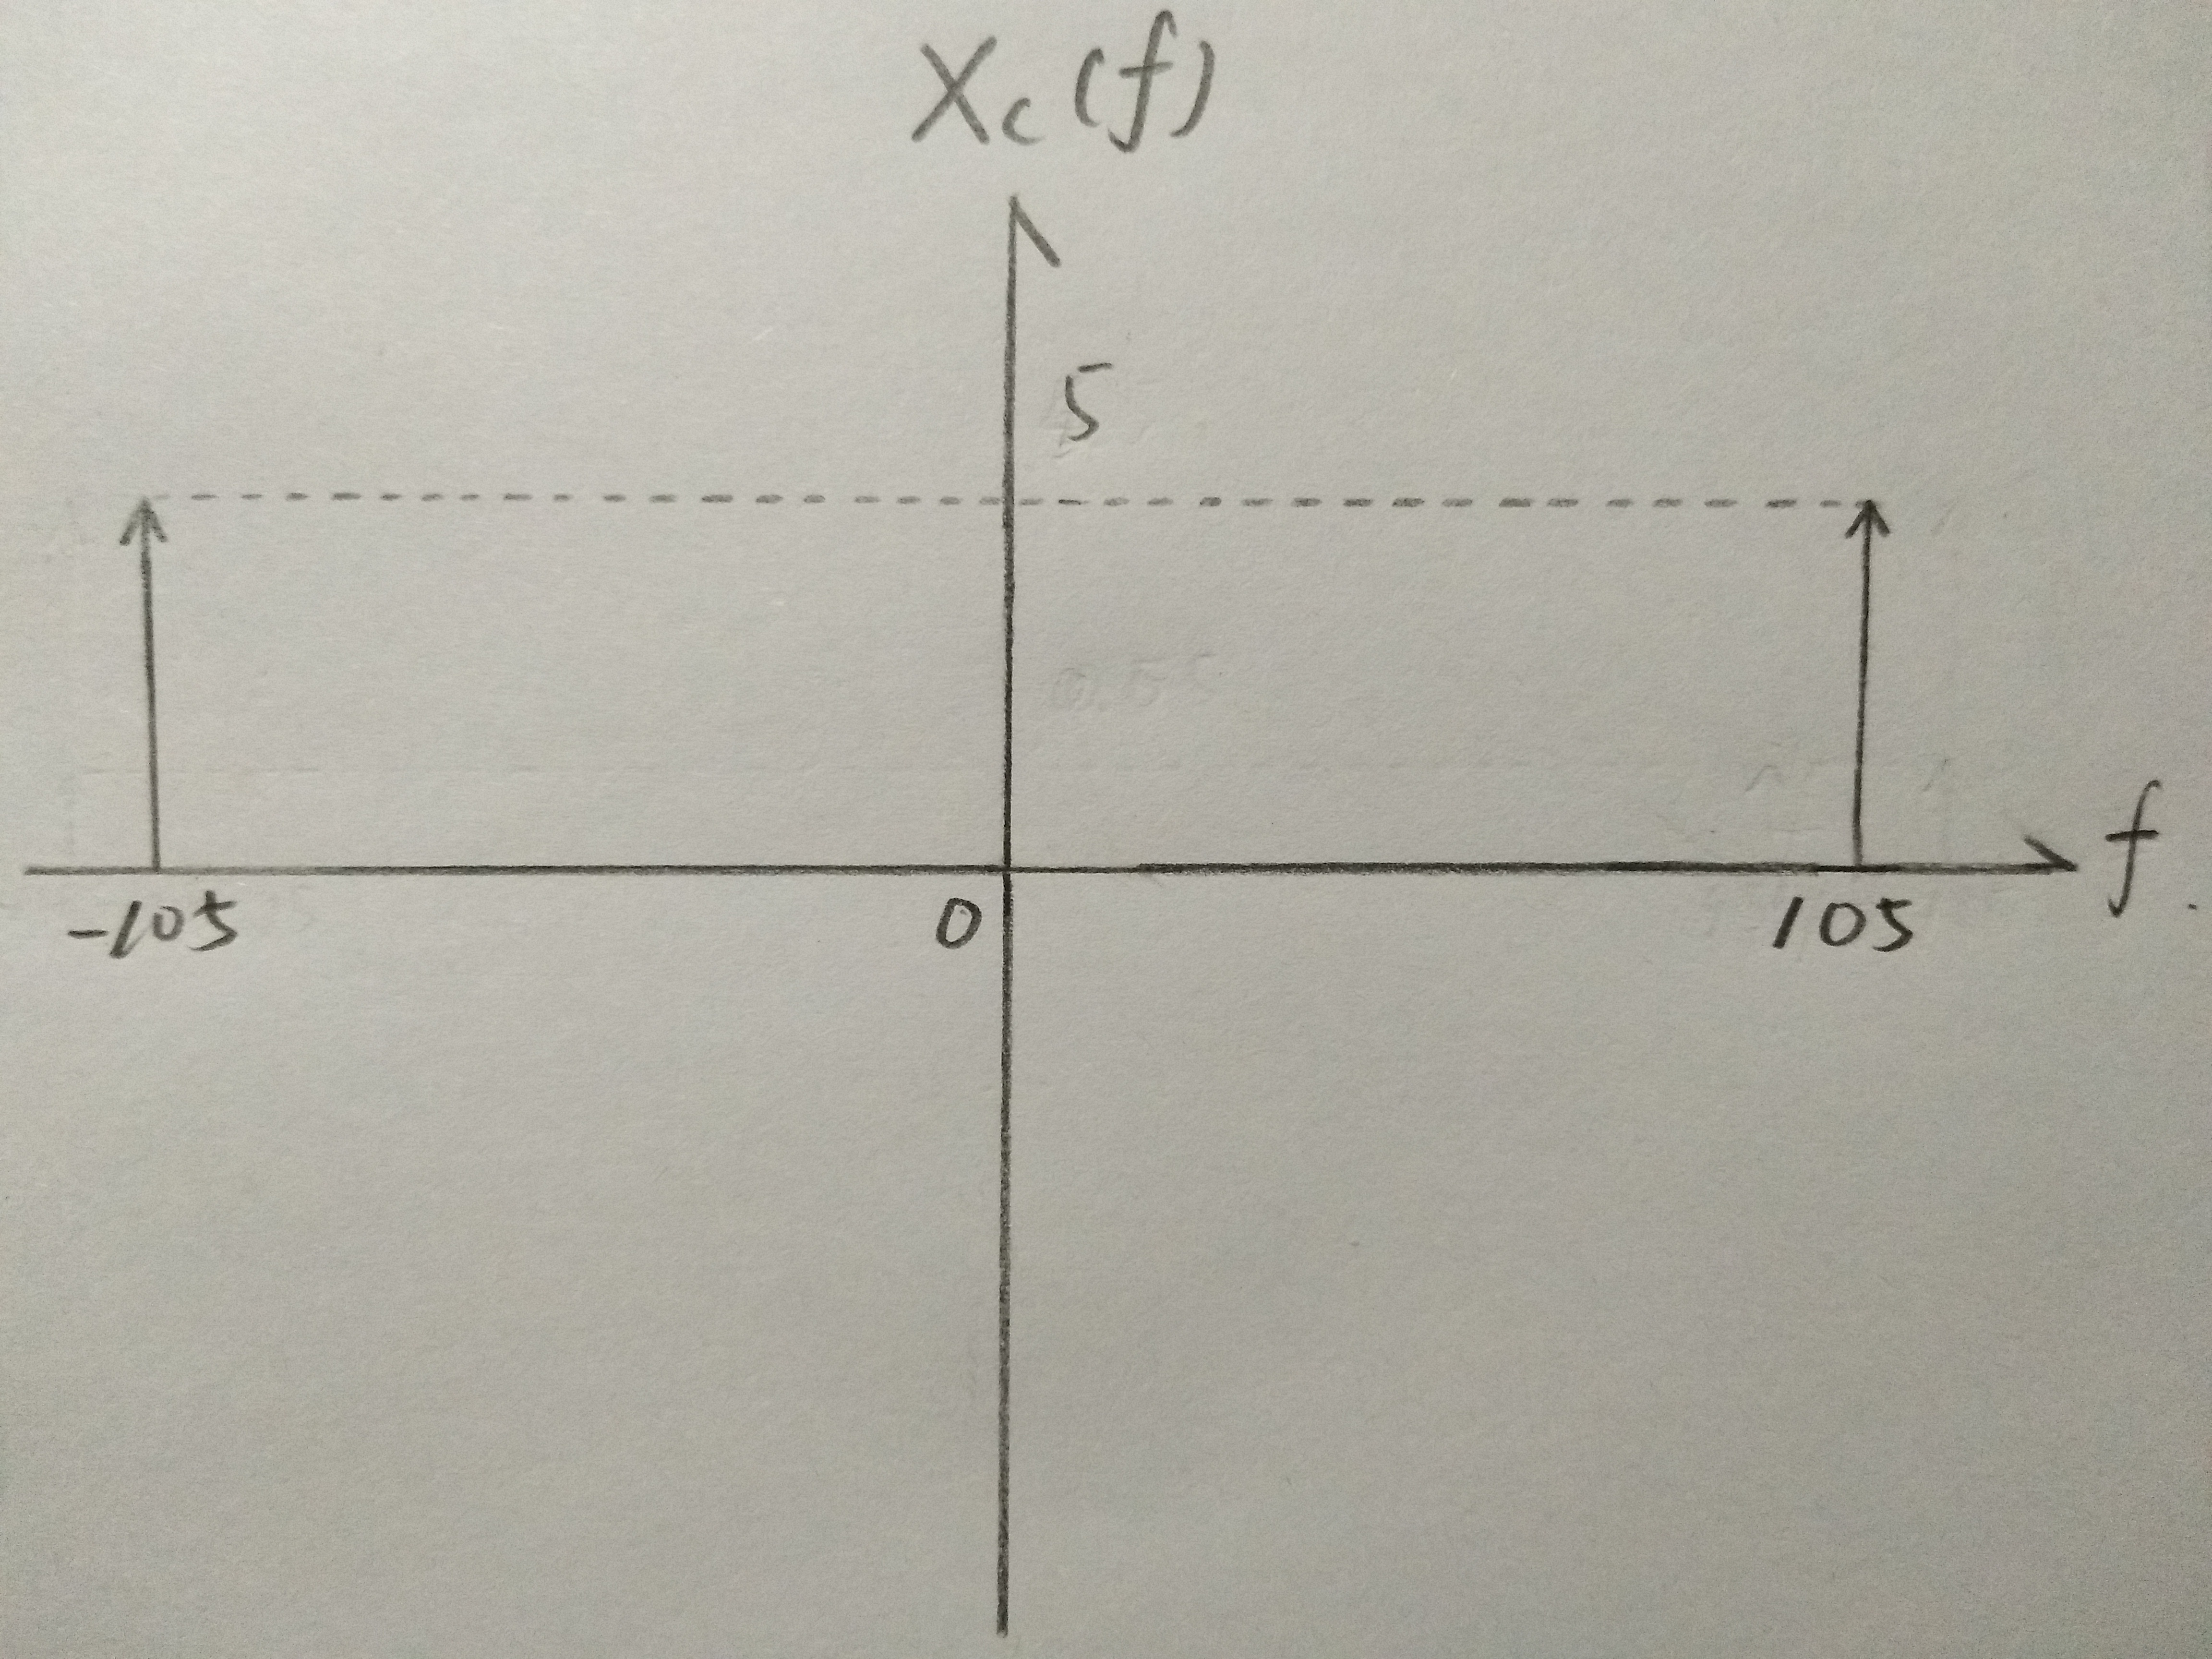
\includegraphics[width=.45\columnwidth]{Assignment-4-Problem-1-3.jpg}
                \label{Assignment-4-Problem-1-3}
            }
            \subfigure[DSB-LC]{
                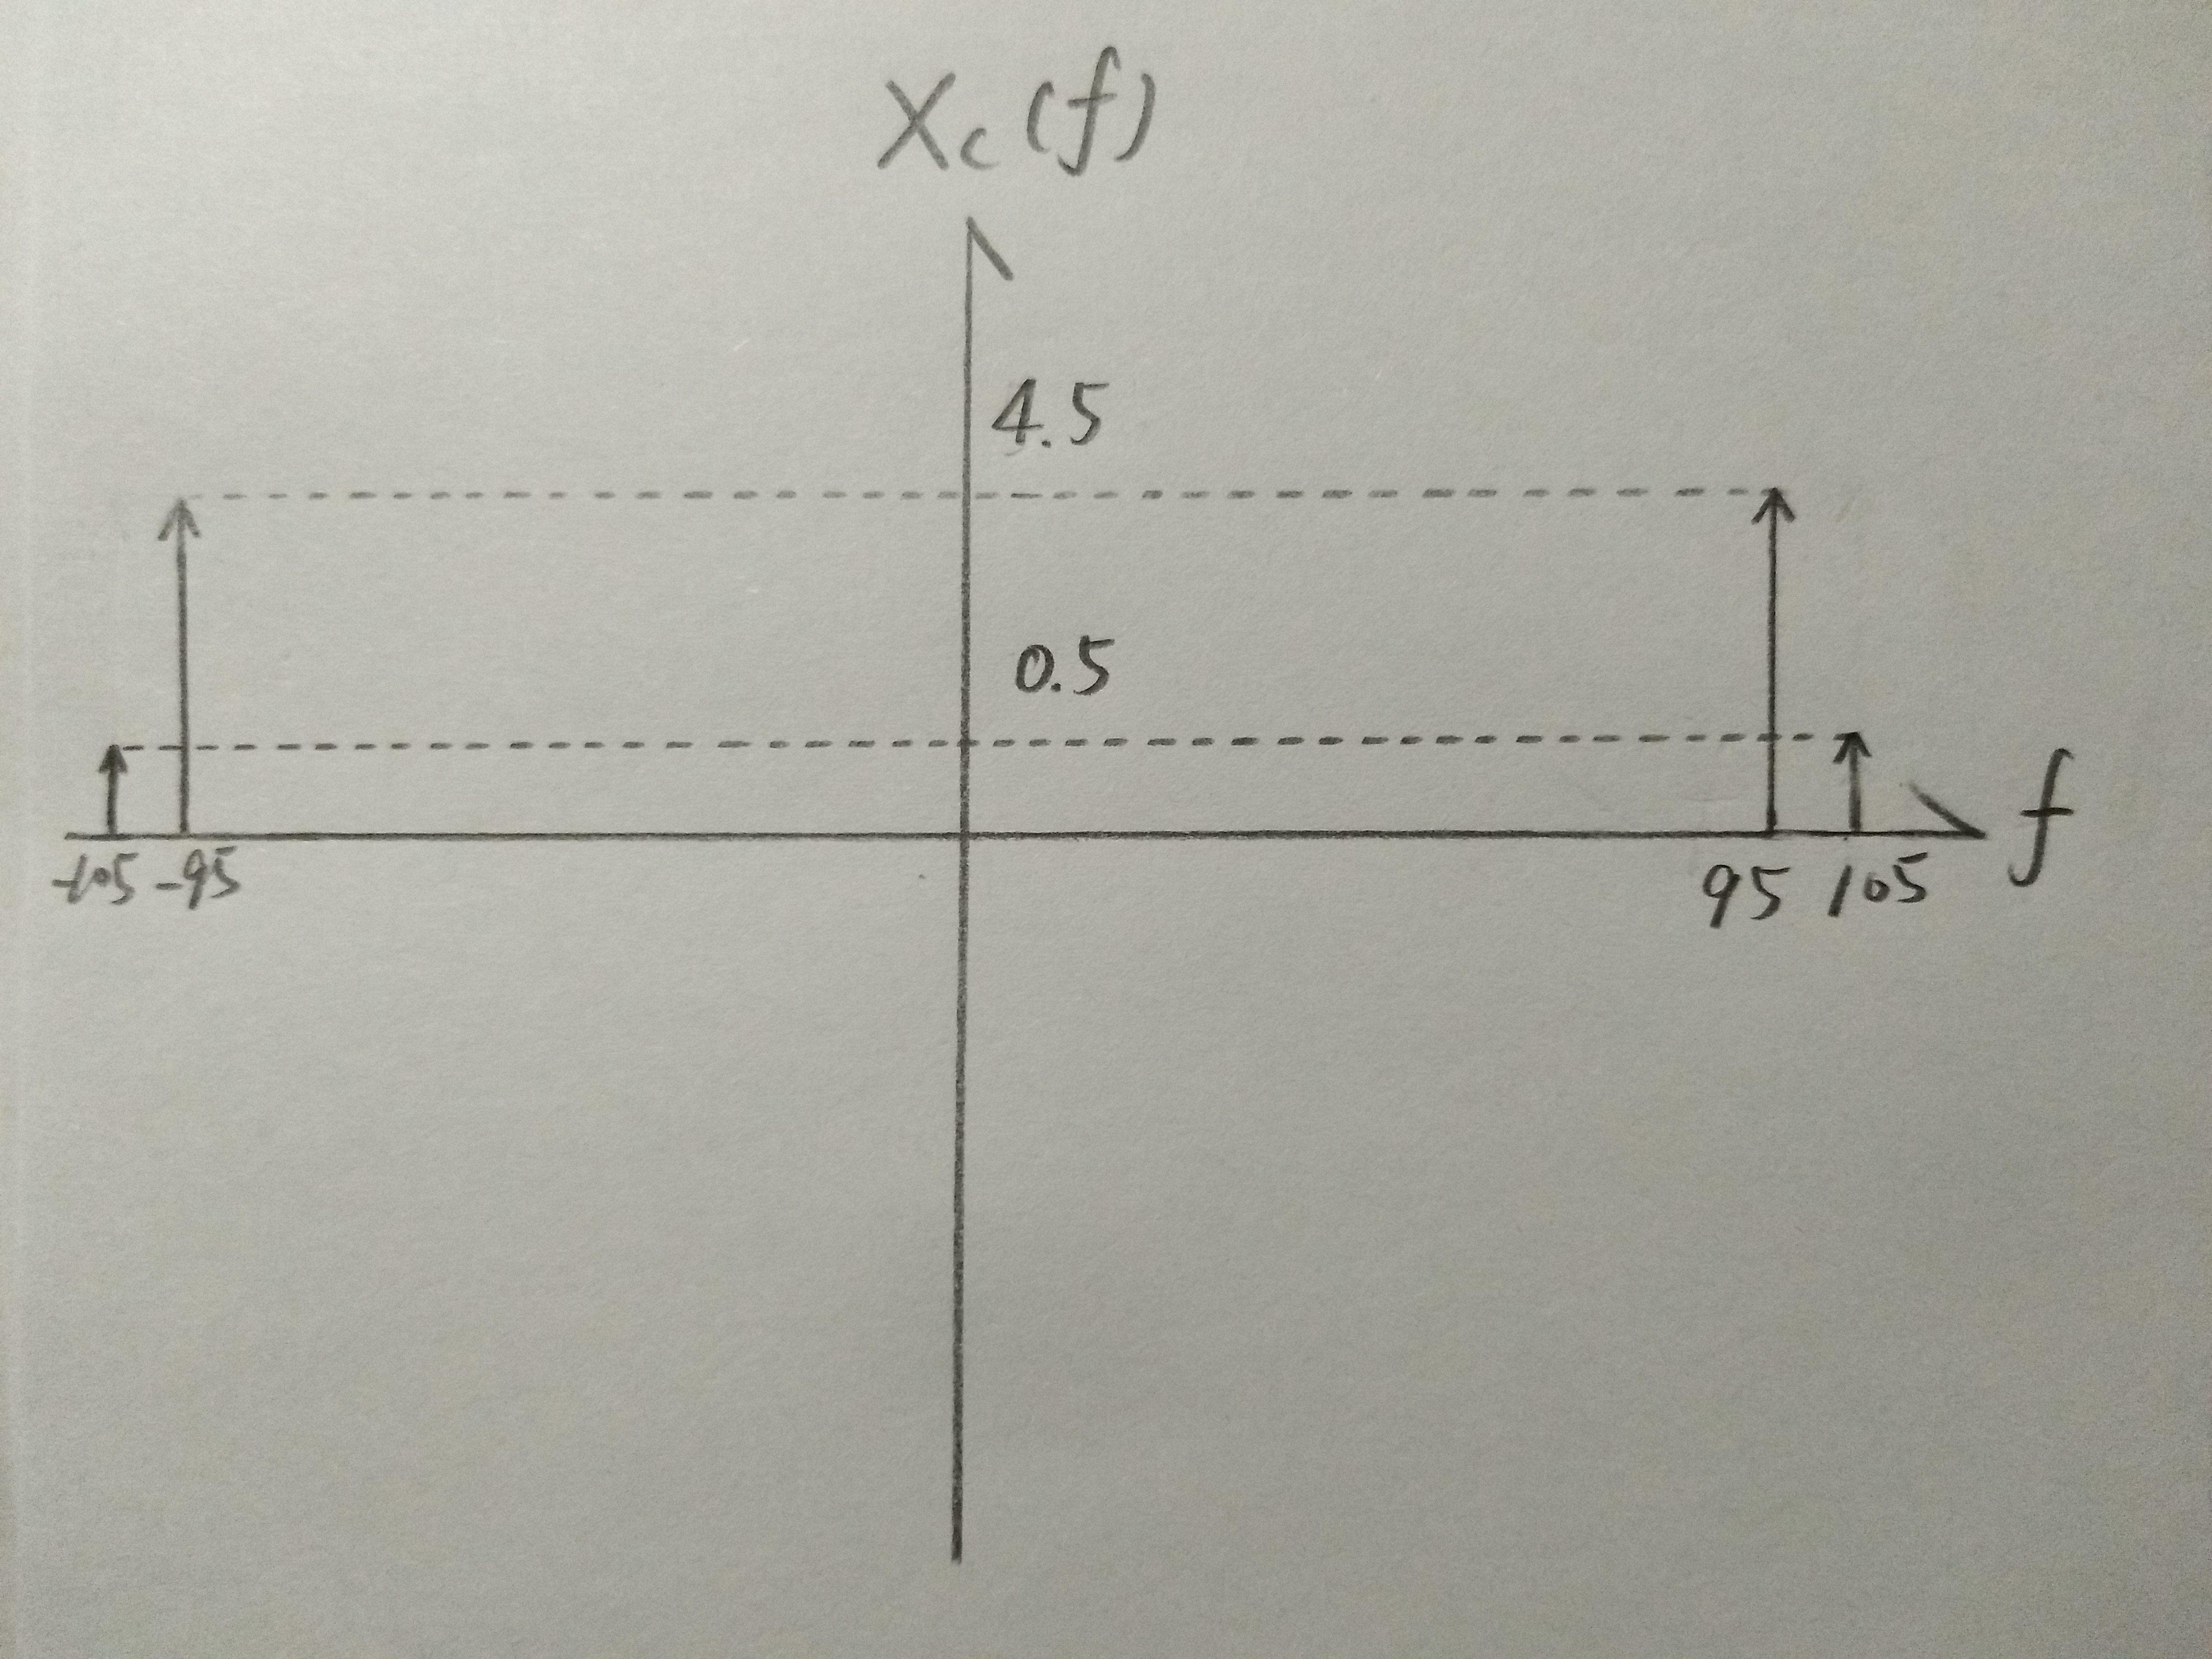
\includegraphics[width=.45\columnwidth]{Assignment-4-Problem-1-4.jpg}
                \label{Assignment-4-Problem-1-4}
            }
            \caption{The spectrum of the modulated signal}
        \end{figure}
    \end{itemize}
\end{sol}
\clearpage

\begin{prob}[DSB-LC or AM, 20 pts]
    An AM (i.e. DSB-LC) modulator has output $x_c(t)=40\cos(400\pi t)+10\cos(360\pi t)+10\cos(440\pi t)$. Determine the modulation index, the carrier power, the sideband power and the transmission efficiency.
\end{prob}
\begin{sol}
    The spectrum of the modulated signal is
    \begin{align}
        X_c(f)=\mathscr{F}[X_c(t)]=20[\delta(f-200)+\delta(f+200)]+5[\delta(f-180)+\delta(f+180)+\delta(f-220)+\delta(f+220)].
    \end{align}
    From the spectrum, we know the carrier frequency of the DSB-LC AM is $f_c=200$ Hz.
    We use phase-coherent demodulation to determine the message signal. Multiplying the output with a local oscillator, we get
    \begin{align}
        \notag x_c(t)\cdot 2\cos(2\pi f_c)=&2[40\cos(400\pi t)+10\cos(360\pi t)+10\cos(440\pi t)]\cos(400\pi t)\\
        =&40[\cos(800\pi t)+1]+10[\cos(40\pi t)+\cos(760\pi t)]+10[\cos(40\pi t)+\cos(840\pi t)],
    \end{align}
    Then we send the signal to a low-pass filter, we get
    \begin{align}
        \text{LP}[x_c(t)\cdot 2\cos(2\pi f_ct)]=&40+20\cos(40\pi t)=A_c\left[1+a\frac{m(t)}{\abs{\min[m(t)]}}\right].
    \end{align}
    Therefore, we get $A_c=40$ and the modulation index
    \begin{align}
        a=\frac{1}{2}.
    \end{align}
    From above, we know the carrier is
    \begin{align}
        C(t)=A_c\cos(2\pi f_ct)=40\cos(400\pi t).
    \end{align}
    The preprocessed message signal is
    \begin{align}
        m_n(t)=\frac{m(t)}{\abs{\min[m(t)]}}=\cos(40\pi t).
    \end{align}
    The carrier power is
    \begin{align}
        P_c=\frac{1}{2}A_c^2=800.
    \end{align}
    The sideband power is
    \begin{align}
        P_s=\frac{1}{2}A_c^2a^2\langle m_n^2(t)\rangle=100.
    \end{align}
    The transmission efficiency is
    \begin{align}
        \mu=\frac{P_s}{P_s+P_c}=\frac{1}{9}.
    \end{align}
\end{sol}

\begin{prob}[Demodulation of SSB, 20 pts]
    \begin{itemize}
        \item[a)] Consider a message signal $m(t)$ containing frequency components at $100$, $200$ and $400$ Hz. This signal is applied to an SSB modulator together with a carrier at $100$ kHz, with only the upper sideband retained. In the coherent detector used to recover $m(t)$, the local oscillator supplies a cosine wave of frequency $100.02$ kHz. Determine the frequency components of the detector output.
        \item[b)] Repeat your analysis, assuming that only the lower sideband is transmitted.
    \end{itemize}
\end{prob}
\begin{sol}
    \begin{itemize}
        \item[a)] Suppose the spectrum of the message signal is
        \begin{align}
            M(f)=\frac{a_1}{2}[\delta(f-100)+\delta(f+100)]+\frac{a_2}{2}[\delta(f-200)+\delta(f+200)]+\frac{a_3}{2}[\delta(f-400)+\delta(f+400)].
        \end{align}
        The spectrum of the SSB modulated signal with only the upper sideband retained is
        \begin{align}
            \notag X_c(f)=&\frac{A_c}{2}\left\{\frac{a_1}{2}[\delta(f-100000-100)+\delta(f+100000+100)]\right.\\
            \notag&\quad+\frac{a_2}{2}[\delta(f-100000-200)+\delta(f+100000+200)]\\
            &\quad\left.+\frac{a_3}{2}[\delta(f-100000-400)+\delta(f+100000+400)]\right\}.
        \end{align}
        The spectrum of the demodulated signal is
        \begin{align}
            \notag D(f)=&\text{LP}[X_c(f-100020)+X_c(f+100020)]\\
            =&\frac{A_c}{2}\left\{\frac{a_1}{2}[\delta(f-80)+\delta(f+80)]+\frac{a_2}{2}[\delta(f-180)+\delta(f+180)]+\frac{a_3}{2}[\delta(f-380)+\delta(f+380)]\right\}.
        \end{align}
        Therefore, the frequency components of the detector output are at $80$ Hz, $180$ Hz and $380$ Hz.
        \item[b)] The spectrum of the SSB modulated signal with only the lower sideband retained is
        \begin{align}
            \notag X_f(f)=&\frac{A_c}{2}\left\{\frac{a_1}{2}[\delta(f-100000+100)+\delta(f+100000-100)]\right.\\
            \notag&\quad+\frac{a_2}{2}[\delta(f-100000+200)+\delta(f+100000-200)]\\
            &\quad\left.+\frac{a_3}{2}[\delta(f-100000+400)+\delta(f+100000-400)]\right\}.
        \end{align}
        The spectrum of the demodulated signal is
        \begin{align}
            \notag D(f)=&\text{LP}[X_c(f-100020)+X_c(f+100020)]\\
            =&\frac{A_c}{2}\left\{\frac{a_1}{2}[\delta(f-120)+\delta(f+120)]+\frac{a_2}{2}[\delta(f-220)+\delta(f+220)]+\frac{a_3}{2}[\delta(f-420)+\delta(f+420)]\right\}.
        \end{align}
        Therefore, the frequency components of the detector output are at $120$ Hz, $220$ Hz and $420$ Hz.
    \end{itemize}
\end{sol}

\noindent\textcolor{red}{Note that the following two problems are two extension problems based on what you have learned on the class.}

\begin{prob}[Square-Law Modulator, 30 pts]
    Consider a square-law modulator, as shown in Figure \ref{Assignment-4-Problem-4}. Assume that the average value of $m(t)$ is zero ($\langle m(t)\rangle=0$), and that the maximum value of $\abs{m(t)}$ is $M$. Also assume that the square-law device in Figure \ref{Assignment-4-Problem-4} is defined by $y(t)=a_1x(t)+a_2x^2(t)$, where $a_1$ and $a_2$ are constants.
    \begin{itemize}
        \item[a)] Write the equation for $y(t)$.
        \item[b)] Assume the bandwidth of the message signal $m(t)$ is $W$. Describe the filter in Figure \ref{Assignment-4-Problem-4}, that yields an AM signal for $g(t)$ with $f_c$ as the carrier frequency. Give the necessary filter type and the carrier frequencies of interest. (Hint: What is the center frequency of the filter, what's the bandwidth of the filter, what's the requirement for the carrier frequency $f_c$ in order to generate an AM signal using square-law modulator. Note that AM signal means DSB-LC modulator signal)
        \item[c)] What's the modulation index of the output AM signal $g(t)$? (Hint: express the modulation index using $a_1$, $a_2$ and $M$)
        \item[d)] What is the advantage of this method of modulation?
    \end{itemize}
    \begin{figure}[h]
        \centering
        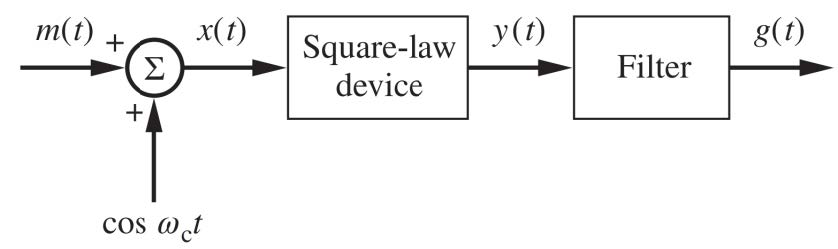
\includegraphics[width=.5\columnwidth]{Assignment-4-Problem-4.jpg}
        \caption{}
        \label{Assignment-4-Problem-4}
    \end{figure}
\end{prob}
\begin{sol}
    \begin{itemize}
        \item[a)] The equation for $y(t)$ is
        \begin{align}
            \notag y(t)=&a_1[m(t)+\cos(\omega_ct)]+a_2[m(t)+\cos(\omega_ct)]^2\\
            \notag=&a_1m(t)+a_1\cos(\omega_ct)+a_2m^2(t)+2a_2m(t)\cos(\omega_ct)+a_2\cos^2(\omega_ct)\\
            =&a_1m(t)+a_2m^2(t)+a_1\left[1+\frac{2a_2}{a_1}m(t)\right]\cos(\omega_ct)+\frac{a_2}{2}[\cos(2\omega_ct)+1].
        \end{align}
        \item[b)] What we want to get is DSB-LC modulator signal:
        \begin{align}
            g(t)=a_1\left[1+\frac{2a_2}{a_1}m(t)\right]\cos(\omega_ct),
        \end{align}
        so we need the carrier frequency to be greater than threefold of the bandwidth of the message signal:
        \begin{align}
            f_c>3W,
        \end{align}
        and we need the center frequency $f_0$ and the bandwidth $B$ of the filter satisfy
        \begin{align}
            f_c+W<f_0+B<2f_c,\quad 2W<f_c-B<f_c-W.
        \end{align}
        One of the proper choices is that the center frequency of the filter equals the carrier frequency and the bandwidth of the filter is greater than the twice of the bandwidth of the message signal and less than $f_c-2W$:
        \begin{align}
            f_0=f_c,\quad 2W<B<2f_c-4W.
        \end{align}
        \item[c)] The output AM signal is
        \begin{align}
            g(t)=a_1\left[1+\frac{2a_2M}{a_1}\frac{m(t)}{M}\right]\cos(\omega_ct)
        \end{align}
        The modulation index of the output AM signal $g(t)$ is
        \begin{align}
            \frac{2a_2M}{a_1}.
        \end{align}
        \item[d)] The advantage of this method of modulation:
        \begin{itemize}
            \item[(1)] This method includes the carrier into the modulated signal, and thus make it easy for envelope detection.
            \item[(2)] This method is relatively easy to realize.
        \end{itemize}
    \end{itemize}
\end{sol}

\begin{prob}[Square-Law Detector, 10 pts]
    Consider a square-law detector as shown in Figure \ref{Assignment-4-Problem-5}, using a nonlinear device whose transfer characteristic is defined by $y(t)=a_1x(t)+a_2x^2(t)$, where $a_1$ and $a_2$ are constants, $x(t)$ is the input, and $y(t)$ is the output. The input consist of the AM wave $x(t)=A_c[1+am_n(t)]\cos\omega_ct$.
    \begin{itemize}
        \item[a)] Write the equation for $y(t)$.
        \item[b)] Find the condition for which the message signal $m(t)$ may be recovered from the $y(t)$. (Hint: What's the ration of the wanted signal to the distortion, and how to keep the ratio large?)
    \end{itemize}
    \begin{figure}[h]
        \centering
        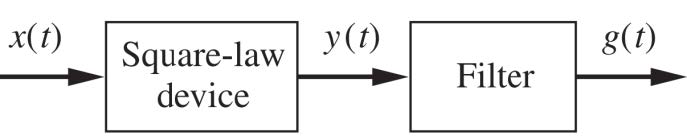
\includegraphics[width=.5\columnwidth]{Assignment-4-Problem-5.jpg}
        \caption{}
        \label{Assignment-4-Problem-5}
    \end{figure}
\end{prob}
\begin{sol}
    \begin{itemize}
        \item[a)] The equation for $y(t)$ is
        \begin{align}
            \notag y(t)=&a_1A_c[1+am_n(t)]\cos\omega_c+a_2A_c^2[1+am_n(t)]^2\cos^2\omega_ct\\
            \notag=&a_1A_c[1+am_n(t)]\cos\omega_ct+a_2A_c^2[1+2am_n(t)+a^2m_n^2(t)]\frac{1+\cos 2\omega_ct}{2}\\
            =&\frac{1}{2}a_2^2A_c^2[1+2am_n(t)+a^2m_n^2(t)]+a_1A_c[1+am_n(t)]\cos\omega_ct+\frac{1}{2}a_2^2A_c^2[1+2am_n(t)+a^2m_n^2(t)]\cos 2\omega_ct
        \end{align}
        \item[b)] We can use a filter that can filter high frequency signal and DC signal. After passing the filter, we can get
        \begin{align}
            g(t)=\frac{1}{2}a_2^2A_c^2am_n(t)[2+am_n(t)].
        \end{align}
        What we want to get is
        \begin{align}
            a_2^2A_c^2am_n(t).
        \end{align}
        The distortion is
        \begin{align}
            \frac{1}{2}a_2^2A_c^2a^2m_n^2(t).
        \end{align}
        The ratio of the wanted signal to the distortion is
        \begin{align}
            \frac{2}{am_n(t)}.
        \end{align}
        Therefore, we can recover $m(t)$ from $y(t)$ when $am_n(t)$ is very large.
    \end{itemize}
\end{sol}
\end{document}